\section{Predictive Modeling \& Decision Making}
\frame{\sectionpage}



\begin{frame}{Supervised Learning Fundamentals}
    \begin{figure}
        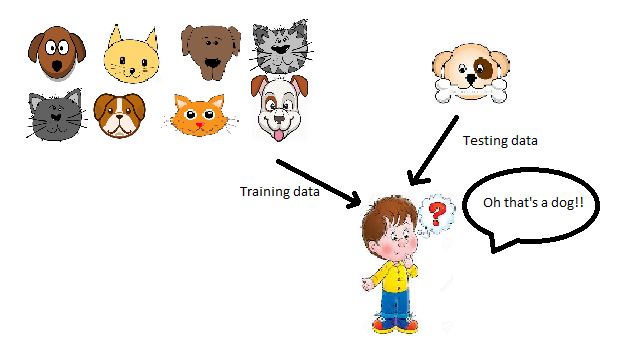
\includegraphics[scale=0.4]{img/supervised_learning_example.png}
        \caption{Supervised Machine Learning. URL: https://medium.com/campusx/machine-learning-from-a-5-year-old-perspective-93278fbf73ce}
    \end{figure}
\end{frame}

\begin{frame}[allowframebreaks]
    \frametitle{Supervised Learning}
    \begin{alertblock}{Mathematical Framework}
        \begin{enumerate}
            \item  Consider a collection of $n$ examples $z_1,\dots, z_n$ represented by a tuple $z_i:= (x_i, y_i)$
         composed by a vector of features $x_i\in \R^n$ and a label $y_i$.\\
      
         \item The objective is to estimate a function $f: X \rightarrow Y$ that maps the observed features into
            their respective label. \\
      
         \item The function is approximated from a set of candidates indexed by a parameter:
          $$
          F = \{ f_{\theta} : \theta \in \Theta\}
          $$
      
         \item The quality of the approximation is measured by defining a loss function $L(\theta)$ that measures
          the distance $l$ between the true value $y_i$ and the predicted values $\hat y_i = f_{\theta}(x_i)$.
      
          $$
              L(\theta):= \sum_{i=1}^n l(y_i, \hat y_i)
          $$
          
          
         \item  The optimization problem then becomes finding 
          
          $$
          \hat \theta = \argmax_{\theta in \Omega} \{ L(\theta)+ \Omega(\theta) \}
          $$
      
        \end{enumerate}
    \end{alertblock}
\end{frame}


\begin{frame}{Time Series Classification}

    \begin{alertblock}{TSC}
\begin{enumerate}
    \item Cutting-tasks are modeled as multivariate time series. A time series is a discrete sequence of data points $\{x_t\}_{t\in \N}$, where each $x_i$ lives in some vector space (e.g. $\R^m$)
    \item Time Series Classification (TSC) is a hard problem, highly dependent on data types and domain context.
\end{enumerate}
    \end{alertblock}
    \begin{alertblock}{TSC}
    Three types of models: Distance-based, Model-based and Feature-based.     
    \end{alertblock}
\end{frame}


\begin{frame}
    \frametitle{TSC Example}
   Visual example of Time series classification. Use tikz. 
\end{frame}

\begin{frame}
    \frametitle{Feature Engineering}
    \begin{alertblock}{Features}
       We considered:
       \begin{enumerate}
           \item Statistical Features.
           \item Ergonomic Threshold Features.
       \end{enumerate}
       The threshold features are randomly sampled from a grid, and selected by evaluating performance on the test set.
    \end{alertblock}
\end{frame}


\begin{frame}{Feature Engineering}
    \begin{alertblock}{Hyperextension Feature}
        The threshold feature $T_1$ is defined as the number of times that the kinematic 
        variable $X$ surpasses a threshold value $\varphi$, indicating the presence of
        hyperextension.
    \end{alertblock}

    \begin{alertblock}{Maximum Exertion Feature}
        The threshold feature $T_2$ is defined as the percentage of the time
        in which the kinematic variable $X$ surpasses a proportion $\gamma \in [0,1]$ of the Maximum
        observed value, indicating the proportion of time in which the worker is performing
        dangerous tasks.
    \end{alertblock}
\end{frame}



\begin{frame}{Performance}
    \begin{alertblock}{Evaluation Metrics}
       \begin{enumerate}
           \item The classifier is evaluated in the test set using evaluation metrics.
           \item Common metrics are Accuracy, Precision and Recall.
           \item In the binary classification case, there are TP, TN, FN and FP. Metrics are calculated acording different aspects of the distirbution.
           \item For the multivariate case, the extension is simple.
       \end{enumerate}
    \end{alertblock}
\end{frame}

\begin{frame}{Performance}
    For each machine learning problem assessing each risk factor we consider different metrics. Accuracy focuses on overall performance, precision focuses in
    reducing false positives and recall focuses on detecting all the negatives.
\end{frame}

\begin{frame}{Performance}
    \begin{table}[H]
        \centering
        \caption{Proposed evaluation metrics for WRMSDs ML problems}
        \begin{tabular}{cc|ccc}
            \toprule
            ML Problem  & Objective & Dataset & Training Evaluation & Test Evaluation \\
            \midrule
            CTC-$6$, CTC-$11$   & Multi-class & $D_1$ & $F_{1(m)}$    &Accuracy\\
            CTC-$2$            & Binary       & $D_2$ &  $F_1$     &Accuracy\\
            KEC-$6^*$, KEC-$11$  & Binary       &  $D_1$ & $F_1$     & Recall \\
            KEC-$2$            & Binary        & $D_2$ & $F_1$     & Recall\\
            PRP                 & Multi-class    & $D_3$ &   $F_{1(m)}$  & Accuracy\\
            \bottomrule
            \multicolumn{5}{l}{$^{*}$: Two versions of KEC task are studied on dataset $D_1$ (6 and 11 cutting-task types);}\\
                \multicolumn{5}{l}{ and one on $D_2$ (2 cutting-task types). However, the problem is still binary (blunt and sharp knife)}\\
        \end{tabular}
        \label{paper_table:evaluation_metrics_wrmsds}
    \end{table}
\end{frame}




